\chapter{Autonomous Navigation}\label{ch:autonomous.navigation}

With all the necessary tools for creating navigation systems in place (environments, their representations and controllers), the next major step in the work is to create and implement autonomous navigation methods.

This chapter presents the different methods studied and the navigation algorithms designed. The various tests carried out were done in simulated environments. Real-world testing is discussed in Chapter \ref{ch:real.world.testing}.

\section{Generic navigation algorithm}

In order to navigate the drone autonomously, a navigation algorithm must be defined. For this, the main steps of a navigation from a starting point to an objective must be clearly defined.

As the drone has a simple representation of its environment (Chapter \ref{ch:environment.representation}), its navigation essentially consists of detecting the key points that compose it. In other words, the drone must be able to detect, in an autonomous way, turns, crossroads and staircases of an environment.

Based on this, an algorithm can be defined. First, the drone must calculate the shortest path from the starting point to the objective, on the basis of its representation of the environment, and extract the corresponding list of key points. Then the drone can take off. As long as the drone has not reached its objective, it takes a picture of its environment and analyzes it to try to detect whether it is a key point or not. Based on this, the drone performs an action and updates its position in its representation of the environment. When the drone has arrived at its objective, it lands.

When the drone moves, it is likely to deviate slightly from its trajectory. It is therefore interesting to also add a system allowing the drone to align itself correctly before continuing its navigation.

This generic algorithm is presented in Algorithm \ref{alg:06.generic.navigation.algorithm}.

\begin{algorithm}[H]
    \begin{algorithmic}[1]
        \Function{navigate}{$start$, $end$}
            \State Let $env$ be the representation of the environment
            \State Let $drone$ be the controller of the drone \\
            \State $path \gets$ \Call{env.path}{$start$, $end$} \Comment{Compute the shortest path}
            \State $keypoints \gets$ \Call{env.keypoints}{$path$} \Comment{Extract key points from the path} \\
            \State \Call{drone.takeoff()}{} \Comment{Take off the drone} \\
            \While{drone has not reach its objective}\label{alg:06.generic.navigation.algorithm.reach.objective}
                \State $picture \gets$ \Call{drone.picture()}{} \Comment{Take a picture}
                \State $type \gets$ \Call{\textcolor{blue}{analyze}}{$picture$} \Comment{Analyze the image} \\
                \If{$type$ is a key point}
                    \State $action \gets$ \Call{get\_action}{$keypoints$} \Comment{Get appropriate action}\label{alg:06.generic.navigation.algorithm.get.action}
                \Else
                    \State \Call{\textcolor{blue}{align}}{$picture$, $drone$} \Comment{Align the drone}
                    \State $action \gets$ move forward
                \EndIf \\
                \State \Call{drone.execute}{$action$} \Comment{Execute the action}
                \State \Call{env.update}{$action$} \Comment{Update position of the drone in environment}
            \EndWhile \\
            \State \Call{drone.land()}{} \Comment{Land the drone}
        \EndFunction
    \end{algorithmic}
    \caption{Generic algorithm for autonomous drone navigation.}
    \label{alg:06.generic.navigation.algorithm}
\end{algorithm}

The actions related to the drone (take-off, image capture, displacement and landing) are performed via the controller (Chapter \ref{ch:controllers}). The actions related to the environment (determination of the shortest path, extraction of key points, updating of the drone's position) are carried out via the representation of the environment (Chapter \ref{ch:environment.representation}).

As the position of the drone in the environment representation is updated each time it moves, in order to determine whether the drone has reached its objective (line \ref{alg:06.generic.navigation.algorithm.reach.objective} of Algorithm \ref{alg:06.generic.navigation.algorithm}), the position of the drone in the environment representation is simply compared to the position of the objective.

\begin{note}
    This method to check if the objective is reached may seem highly inaccurate, but it actually provides good results. Although the position of the drone is approximated as it moves, it is updated accurately each time a key point is detected (Section \ref{sec:05.drone.position}). Unless the objective is very far from a key point, the position reached by the drone is always very close to its intended objective. However, it would be possible, in a future work, to improve the landing position of the drone by using, for example, distinct landmarks to detect in the environment.
\end{note}

Determining the action to be taken when a key point has been detected (line \ref{alg:06.generic.navigation.algorithm.get.action} of Algorithm \ref{alg:06.generic.navigation.algorithm}) is done simply by consulting the list of key points (and their associated actions) extracted from the path. The first key point detected will give rise to the first action in the list, the second key point to the second action in the list, etc.

Only the actions \textsc{\textcolor{blue}{align}} and \textsc{\textcolor{blue}{analyze}} need to be determined in order to define a functional algorithm. The rest of this chapter therefore presents the architecture adopted to implement this generic algorithm, the methods used to implement the alignment and analysis actions and the various results obtained.

\section{Architecture}\label{sec:06.architecture}

The different navigation algorithms all share a common structure (Algorithm \ref{alg:06.generic.navigation.algorithm}), only the methods \textsc{\textcolor{blue}{align}} and \textsc{\textcolor{blue}{analyze}} are different. In order to be able to carry out multiple algorithms while keeping a comprehensible and easily maintainable solution, a particular architecture has been adopted.

Each of the methods (\textsc{\textcolor{blue}{align}} and \textsc{\textcolor{blue}{analyze}}) is implemented via a \emph{module}. A module is therefore simply a small algorithm that allows a specific task to be carried out on the basis of information provided by the drone (\eg{} a picture).

The generic navigation algorithm is implemented via an abstract class (\texttt{NavAlgorithm}). Each algorithm created inherits from this class and is composed of one or more modules allowing the implementation of the different methods (alignment and analysis).

The general architecture, with some generic examples, is shown in Figure \ref{fig:06.navigation.algorithms.architecture}.

\begin{figure}[H]
    \centering
    \begin{tikzpicture}
        \umlclass[type=abstract]{NavAlgorithm}{
            env : Environment \\
            drone : Controller
        }{
            \umlvirt{navigate($start$, $end$) : void} \\
            \textcolor{blue}{align}($picture$, $drone$) : void \\
            \textcolor{blue}{analyze}($picture$) : bool \\
        }
        \umlsimpleclass[x=-5.5, y=-4, fill=green!20]{NavAlgorithmOne}
        \umlsimpleclass[x=-5.5, y=-5, fill=blue!20]{ModuleOne}
        \umlsimpleclass[x=0, y=-4, fill=green!20]{NavAlgorithmTwo}
        \umlsimpleclass[x=0, y=-5, fill=blue!20]{ModuleOne}
        \umlsimpleclass[x=0, y=-6, fill=blue!20]{ModuleTwo}
        \umlsimpleclass[x=5.5, y=-4, fill=green!20]{NavAlgorithmThree}
        \umlsimpleclass[x=5.5, y=-5, fill=blue!20]{ModuleTwo}
        \umlsimpleclass[x=5.5, y=-6, fill=blue!20]{ModuleThree}
        \umlimpl[geometry=-|]{NavAlgorithm}{NavAlgorithmOne}
        \umlimpl[geometry=-|]{NavAlgorithm}{NavAlgorithmTwo}
        \umlimpl[geometry=-|]{NavAlgorithm}{NavAlgorithmThree}
    \end{tikzpicture}
    \caption{General architecture adopted to design multiple navigation algorithms.}
    \label{fig:06.navigation.algorithms.architecture}
\end{figure}

Such an architecture has the advantage of allowing the very easy creation of several algorithms by simply combining one or more modules while avoiding code redundancy in the different implementations.

\section{Alignment}

This section concerns the creation of modules used to align the drone (\textsc{\textcolor{blue}{align}}).

In a perspective view of an environment (for example, a picture), the lines parallel to each other no longer appear parallel but all converge at a point called the \emph{vanishing point} (Figure \ref{fig:06.vanishing.point.example}).

\begin{figure}[H]
    \centering
    \includegraphics[width=0.6\textwidth]{resources/png/06/vanishing-point/example.png}
    \caption{Example of a vanishing point (in blue) in a corridor image. The parallel lines (in the real world) are represented in red.}
    \label{fig:06.vanishing.point.example}
\end{figure}

The vanishing point is frequently used when moving a robot. The idea is to make sure that this point is always in the center of the image so that the robot follows a straight trajectory, facing the horizon.

The generic alignment procedure used in this work is described in Algorithm \ref{alg:06.vanishing.point.alignment}, with $\delta$ being the maximum allowed deviation from the center of the image.

\begin{algorithm}[H]
    \begin{algorithmic}[1]
        \Function{\textcolor{blue}{align}}{$picture$, $drone$}
            \State Let $\delta$ be a tolerance. \\
            \State $cx, cy \gets$ \Call{center}{$picture$} \Comment{Get center position of the image}
            \State $vx, vy \gets$ \Call{vanishing\_point}{$picture$} \Comment{Get vanishing point} \\
            \While{$vx < cx - \delta$ or $vx > cx + \delta$}
                \If{$vx < cx - \delta$}
                    \State \Call{drone.rotate}{$left$}
                \EndIf \\
                \If{$vx > cx + \delta$}
                    \State \Call{drone.rotate}{$right$}
                \EndIf \\
                \State $picture \gets$ \Call{drone.picture()}{} \Comment{Take a new picture}
                \State $vx, vy \gets$ \Call{vanishing\_point}{$picture$} \Comment{Get new vanishing point}
            \EndWhile
        \EndFunction
    \end{algorithmic}
    \caption{Generic procedure for aligning the drone using the vanishing point.}
    \label{alg:06.vanishing.point.alignment}
\end{algorithm}

This algorithm first computes the positions of the center point of the image and the vanishing point. It then compares these positions, according to a tolerance $\delta$, to determine if the drone has to rotate left, rotate right or do nothing (because it is sufficiently well aligned). While the drone is not aligned, it continues to take picture and analyzes it. No vertical correction is computed because, as explained in Section \ref{sec:05.occupancy.grid}, the drone only rarely moves up or down (only for staircases) and, practically, it successfully keeps its altitude without (significant) deviation.

The tolerance $\delta$ can be set dynamically according to the dimensions of the image and the method used. The different adjustment actions are performed via the drone controller. In this work, small rotations (left or right) of $\SI{5}{\degree}$ have been used.

\begin{note}
    When the detected vanishing point seems completely wrong (\eg{} if the detected vanishing point is in a corner of the image), the alignment procedure is not applied in order not to lead the drone into an inconsistent position.
\end{note}

To have a functional alignment procedure, the detection of the vanishing point has to be defined (\textsc{vanishing\_point} in Algorithm \ref{alg:06.vanishing.point.alignment}). Several vanishing point detection methods have been tested: two methods working with line detection and one method working with a Deep Learning model.

\subsection{Line detection}\label{sec:06.line.detection}

Since the vanishing point is at the intersection of the parallel lines (in the real world), a first method consists in detecting these lines and compute their intersection.

The detection of the lines of an image is a well-known application in Computer Vision. Although many methods exist, it is certainly not an easy problem: the results are very sensitive to the quality of the image, variations in brightness, colors, etc. It is then difficult to design an algorithm robust to all possible variations.

In this work, the drone moves in corridors, we can therefore make some simplifying assumptions: in the vast majority of images, only one vanishing point will be present and the vanishing point will generally be the intersection of 4 lines representing the boundaries between the walls, the floor and the ceiling.

\subsubsection{Detection via classical methods}

The first method implemented uses classical Computer Vision techniques to detect edges and lines. This method will be called \texttt{VPClassic} and is described below.

\begin{enumerate}
    \item A bilateral filter is applied to the image. This filter replaces the value of each pixel with a weighted average of the intensities of neighboring pixels \cite{wikipedia2021bilateralfilter}. The resulting image preserves its shapes and contours but is smoother; thus reducing noise.
    \item A Canny filter \cite{canny1986computational} is then applied to extract the edges of the image. This filter first applies a Gaussian filter to remove noise and then computes gradient, using convolution masks, to get the intensity of each point. It finally applies some post processing operations to only keep points that belong to edges.
    \item Based on the previously extracted edges, the lines are calculated using a probabilistic Hough transform \cite{kiryati1991probabilistic}. The resulting lines are represented by segments with given $x$ and $y$ endpoints.
    \item The resulting lines are filtered, based on the $x$ coordinates of their endpoints, to remove all those that are vertical (or nearly vertical).
    \item Finally, the vanishing point is calculated based on the intersections of the remaining lines. However, it is (very) possible that more lines than necessary are presented, including lines that are not needed for the vanishing point calculation, which may lead to an incorrect result. Furthermore, as the detection is not perfect, not all lines may intersect at a specific point.

    To overcome this problem, a method inspired by \cite{github2019vanishingpointdetection} was used: the image is separated into a grid and the intersections contained in each cell of the grid are counted. The cell with the most intersections is considered to be the one containing the vanishing point. This method does not give the exact coordinates of the vanishing point, but an area, more or less precise depending on the size of the grid, in which it is located. The coordinates of the vanishing point can be approximated by taking the coordinates of the center point of the cell.
\end{enumerate}

An example of the results obtained with this method is shown in Figure \ref{fig:06.vpclassic.example}. The determined vanishing point is located in the green cell in Figure \ref{fig:06.vpclassic.example.cell}.

\begin{figure}[H]
    \centering
    \begin{subfigure}{0.49\textwidth}
        \centering
        \includegraphics[width=\textwidth]{resources/png/06/vanishing-point/vpclassic/0.png}
        \caption{Bilateral filter}
        \vspace{0.5em}
    \end{subfigure}
    \hfill
    \begin{subfigure}{0.49\textwidth}
        \centering
        \includegraphics[width=\textwidth]{resources/png/06/vanishing-point/vpclassic/1.png}
        \caption{Canny filter}
        \vspace{0.5em}
    \end{subfigure}
    \begin{subfigure}{0.49\textwidth}
        \centering
        \includegraphics[width=\textwidth]{resources/png/06/vanishing-point/vpclassic/2.png}
        \caption{Filtered Hough transform}
    \end{subfigure}
    \hfill
    \begin{subfigure}{0.49\textwidth}
        \centering
        \includegraphics[width=\textwidth]{resources/png/06/vanishing-point/vpclassic/3.png}
        \caption{Extracted vanishing point}
        \label{fig:06.vpclassic.example.cell}
    \end{subfigure}
    \caption{Example of results obtained via the \texttt{VPClassic} vanishing point detection method.}
    \label{fig:06.vpclassic.example}
\end{figure}

\begin{note}
    The lengths of the detected lines could have been taken into account to get more information, for example the distance to the end of the corridor (the smaller the lines, the closer to the end). However, the algorithm does not always detect the whole line (see Figure \ref{fig:06.vpclassic.example}, only small parts of the lines were detected), making this procedure very unstable and thus difficult to use in practice.
\end{note}

\subsubsection{Detection via edgelets and RANSAC}

The detection of the vanishing point being a common problem, the scientific literature is rich in various methods. Another interesting one working with \emph{edgelets} (a triplet, composed of a location, a direction and a strength, representing the features of an edge) and \emph{RANSAC} has been implemented, inspired from the work of \textcite{chaudhury2014auto} and adapted from the implementation of \cite{github2020automatedrectification}. The main idea is to no longer work directly with line detection but with edgelets and to use RANSAC, robust to noise and outliers, to vote for the best candidate at the vanishing point.

This second method will be called \texttt{VPEdgelets}. An example of result is shown in Figure \ref{fig:06.vpedgelets.example}. The obtained vanishing point is represented by a red dot.

\begin{figure}[H]
    \centering
    \includegraphics[width=0.7\textwidth]{resources/png/06/vanishing-point/vpedgelets.png}
    \caption{Example of obtained result via the \texttt{VPEdgelets} vanishing point detection method.}
    \label{fig:06.vpedgelets.example}
\end{figure}

\subsubsection{Evaluation}

Although the obtained results with these two methods seem to be very good on the examples, it is interesting to see how well they really perform. For this purpose, two series of $\num{50}$ images (one per simulated environment) have been collected (by manually controlling the drone in the environments). These $\num{100}$ images are such that the vanishing point is at the most varied locations possible. Some examples are given in Figure \ref{fig:06.vanishing.point.evaluation.examples}.

\begin{figure}[H]
    \centering
    \begin{subfigure}{0.32\textwidth}
        \centering
        \includegraphics[width=\textwidth]{resources/png/06/vanishing-point/evaluation/0.png}
        \vspace{0.5em}
    \end{subfigure}
    \hfill
    \begin{subfigure}{0.32\textwidth}
        \centering
        \includegraphics[width=\textwidth]{resources/png/06/vanishing-point/evaluation/1.png}
        \vspace{0.5em}
    \end{subfigure}
    \hfill
    \begin{subfigure}{0.32\textwidth}
        \centering
        \includegraphics[width=\textwidth]{resources/png/06/vanishing-point/evaluation/2.png}
        \vspace{0.5em}
    \end{subfigure}
    \begin{subfigure}{0.32\textwidth}
        \centering
        \includegraphics[width=\textwidth]{resources/png/06/vanishing-point/evaluation/3.png}
    \end{subfigure}
    \hfill
    \begin{subfigure}{0.32\textwidth}
        \centering
        \includegraphics[width=\textwidth]{resources/png/06/vanishing-point/evaluation/4.png}
    \end{subfigure}
    \hfill
    \begin{subfigure}{0.32\textwidth}
        \centering
        \includegraphics[width=\textwidth]{resources/png/06/vanishing-point/evaluation/5.png}
    \end{subfigure}
    \caption{Examples of images collected for the evaluation of vanishing point detection methods.}
    \label{fig:06.vanishing.point.evaluation.examples}
\end{figure}

Each of the images was annotated with its vanishing point using an annotation tool developed for this work. The tool allows, with a simple mouse click, to select the location of the vanishing point on the image and to save its $x$ and $y$ coordinates.

To evaluate the methods, the coordinates of the vanishing points detected were compared to the manually annotated vanishing points. As manual annotation is not necessarily the most accurate, the evaluation was done by simply comparing whether the coordinates found by the method lie within a zone, of fixed radius (set to one tenth of the width of the image in this work), around the annotated vanishing point. The mean execution time per image of each method, in seconds, was also evaluated. The obtained results are presented in Table \ref{tab:06.vanishing.point.evaluation.results}.

\begin{table}[H]
    \centering
    \begin{tabular}{|l|c|c|}
        \hline
        \textbf{Method} & \textbf{Score} (over 100) & \textbf{Mean execution time} (s) \\ \hline
        \hline
        \texttt{VPClassic} & $\num{93}$ & $\num{0.04}$ \\ \hline
        \texttt{VPEdgelets} & $\num{79}$ & $\num{0.31}$ \\ \hline
    \end{tabular}
    \caption{Results obtained with the evaluation of the vanishing point detection methods.}
    \label{tab:06.vanishing.point.evaluation.results}
\end{table}

The obtained results show that the \texttt{VPClassic} method obtains a better score in terms of detection and a much better mean execution time per image. For these reasons, this method will be kept to create a first module implementing the \textsc{\textcolor{blue}{align}} method (with the deviation $\delta$ set to one twenty-fifth of the image width). A small example of utilization of this module is shown in a video available via the following link: \url{https://youtu.be/oSyHeMTe4y8}.

\subsection{Deep Learning}

Inspired by the work of \textcite{chang2018deepvp}, a Deep Learning model has been used to predict the vanishing point of an image. More precisely, the image is discretized into a grid of a given size and the goal is to determine in which cell the vanishing point is located. The problem then becomes a classification problem: the Deep Learning model infers a probability for each cell indicating the chance that the vanishing point is located there. The coordinates of the center point of the cell with the highest probability is then selected as the vanishing point location.

The more cells the grid contains, the more accurate the vanishing point location will be, but the harder the classification will be (because the number of cells represent the number of possible classes). In this work, being a good compromise between precision, ease and speed, a grid of $\num{5} \times \num{5}$ was chosen (the width and height of each cell are the width and height of the image divided by $\num{5}$).

\subsubsection{Data set}

A data set of $\num{1052}$ images (of size $\num{320} \times \num{180}$ pixels) with annotations has been created. The images are as varied as possible so that the network learns to detect vanishing points at various positions.

The images were collected by manually controlling the drone, and automatically taking pictures at a fixed interval of $\SI{0.5}{\second}$, in the environment and slightly varying its orientation from time to time in a random fashion. An automatic solution to collect the images was considered but not retained (more details in Section \ref{sec:06.image.classification}).

The vanishing point of each of the images was first manually annotated using the previously mentioned tool. The image was then discretized into a grid and the cell containing the vanishing point was marked. More formally, the annotation associated with an image $i$ is a binary vector $y_i$ containing $\num{24}$ zeros and $\num{1}$ one indicating the cell containing the vanishing point. The data set was then separated into a training set of $\num{736}$ images and a testing set of $\num{316}$ images.

\subsubsection{Model}

Being already implemented for classification purposes (see later in Section \ref{sec:06.image.classification}), the model used is a pre-trained version of DenseNet-161 \cite{simonyan2014very}. The original output layer has been replaced by three convolutional layers as well as a linear layer and a Softmax activation function. The detailed architecture can be found in Appendix \ref{ch:neural.networks.architectures}.

\subsubsection{Training}

The model was trained via a \emph{Mean Square Error} (MSE) loss function (because this loss was also already implemented for classification purposes, see Section \ref{sec:06.image.classification}) and an \emph{Adam} \cite{kingma2014adam} optimizer (with a learning rate of $\num{0.001}$) during $\num{30}$ epochs with batches of $\num{8}$ images.

In order to improve the robustness of the model, \emph{data augmentation} was performed. This process consists in applying a random transformation to the image given as input to the network so that the latter is not specific to the characteristics of the images (mainly, its colors). In this work, 5 transformations were implemented: no modification, blur, edge enhance, smooth and color jitter (randomly change the brightness, contrast, saturation and hue).

The evolution of the loss function during training is shown in Figure \ref{fig:06.vpdeeplearning.mse.loss}.

\begin{figure}[H]
    \centering
    \includegraphics[width=0.7\textwidth]{resources/pdf/06/vanishing-point/vpdeeplearning/mse-loss.pdf}
    \caption{Evolution of the MSE loss function during the training of the DenseNet-161 model for the vanishing point detection problem.}
    \label{fig:06.vpdeeplearning.mse.loss}
\end{figure}

We observe that the loss function well decreases over the epochs and converges toward $\num{0}$, which is expected for a good model (see Section \ref{sec:02.deep.learning.basics}). In order to be sure that this was not a lucky case, several trainings were performed: all gave similar results (the same verification is performed for other trainings mentioned in this report).

\begin{note}
    As the network is only trained on images from one or two different environments, it is likely that it slightly overfits these environments (be too specific). This is actually not a big problem as the drone performs its test flights in these environments. However, a \emph{validation set} could have been used to properly quantify the overfitting.
\end{note}

\subsubsection{Evaluation}

Being a classification problem, a \emph{confusion matrix} can be computed. The latter is a matrix that measures the quality of a classification.

To better understand what is a confusion matrix, let's imagine a binary classification problem: each image can be of specified class (for example, a \enquote{car}) or not. Each line of the matrix corresponds to a real class (the class associated to each image of the testing set, in this example, \enquote{car} or \enquote{not car}) and each column to a predicted class (the same classes, but predicted by the model). The cell located at line $i$ and column $j$ represents the number of elements whose real class is $i$ and whose predicted class by the model is $j$. The different cells (four in total) have specific names:

\begin{itemize}
    \item True Positive (TP): an image whose real class is \enquote{car} and predicted class is also \enquote{car};
    \item True Negative (TN): an image whose real class is \enquote{not car} and predicted class is also \enquote{not car};
    \item False Positive (FP): an image whose real class is \enquote{not car} but predicted class is \enquote{car};
    \item False Negative (FN): an image whose real class is \enquote{car} but predicted class is \enquote{not car}.
\end{itemize}

Based on these measures, two metrics, called \emph{precision} and \emph{recall} \cite{hossin2015review}, can be obtained via
\begin{equation*}
    precision = \frac{TP}{TP + FP}, \quad recall = \frac{TP}{TP + FN}
\end{equation*}
The precision represents how many of the positively classified were relevant and the recall represents how good the model is at detecting the positives. Is is important to use at least two metrics because a single metric can be easily fooled if the model predicts, for example, always the same class for all input images.

These metrics, popular to evaluate a classification problem, were used to evaluate the model.

As the classification problem has multiple classes and is totally unbalanced (there are not the same number of images of each class in the data set; in other words, there are not the same number of images for each possible cell of the vanishing point), versions of the metrics weighted according to the occurrence of each class were used (it calculates metrics for each class, and find their average weighted by the number of true instances for each class). The closer these metrics are both to $1$, the better the classification.

The model obtains, on the testing set, a precision of $\num{0.96}$ and a recall of $\num{0.94}$. The mean inference time of the model is $\SI{0.24}{\second}$. These results seem to show a very good performance of the network. To illustrate them, some practical tests were carried out (Figure \ref{fig:06.vpdeeplearning.results.examples}).

\begin{figure}[H]
    \centering
    \begin{subfigure}{0.32\textwidth}
        \centering
        \includegraphics[width=\textwidth]{resources/png/06/vanishing-point/vpdeeplearning/results/0.png}
    \end{subfigure}
    \hfill
    \begin{subfigure}{0.32\textwidth}
        \centering
        \includegraphics[width=\textwidth]{resources/png/06/vanishing-point/vpdeeplearning/results/1.png}
    \end{subfigure}
    \hfill
    \begin{subfigure}{0.32\textwidth}
        \centering
        \includegraphics[width=\textwidth]{resources/png/06/vanishing-point/vpdeeplearning/results/2.png}
    \end{subfigure}
    \caption{Examples of obtained results using the trained DenseNet-161 model for vanishing point detection.}
    \label{fig:06.vpdeeplearning.results.examples}
\end{figure}

Although not extremely accurate (this is impossible given the chosen size of the grid), the obtained results are very convincing. They seem to be sufficient to allow a correct alignment of the drone. Moreover, the trained model has also been evaluated on the $\num{100}$ images used to evaluate the \texttt{VPClassic} and \texttt{VPEdgelets} methods (these images are not coming from the training set). It obtains a score of $\num{100}$ vanishing points detected over $\num{100}$, which is a very impressive result showing the robustness and efficiency of a Deep Learning model.

For these reasons, this method, that will be called \texttt{VPDeepLearning}, will be kept to create a second module implementing the \textsc{\textcolor{blue}{align}} method (with the deviation $\delta$ fixed at the width of a cell).

\section{Key points detection}

This section concerns the creation of modules used to analyze images and detect key points (\textsc{\textcolor{blue}{analyze}}).

After the creation of modules allowing the alignment step of the drone, this work continues by focusing on the most important step of the navigation algorithm (Algorithm \ref{alg:06.generic.navigation.algorithm}): the detection of key points (turns, crossroads and staircases) based on images captured by the drone.

For this, several methods were tested. Inspired by the different works using Deep Learning models (Chapter \ref{ch:sota}) to process images, a method for classifying images via a Deep Learning model was studied. Deep Learning models were also evaluated to perform depth estimation. Finally, the use of markers, popular in the field of robotics, was tested.

\subsection{Image classification}\label{sec:06.image.classification}

Inspired by the work of \textcite{padhy2018deep}, this method allows the detection of key points of an environment based on a classification of images captured by the drone via a Deep Learning model.

In their work, the authors used the DenseNet-161 network and trained it to classify each image of a defined path in a specific action (\enquote{move forward}, \enquote{turn left}, etc.). This implies that a training of the model forces the drone to always follow the same trajectory.

In this work, this idea has been taken up again but in a generalized way. Instead of associating a precise action to each image, the model performs a simple binary classification (\enquote{key point} or \enquote{not key point}).

\subsubsection{Data sets}

To create data sets for training the model, the drone was manually piloted in the simulated environments by capturing images at regular intervals (every $\SI{0.1}{\second}$ for this task). Each set of images collected was manually annotated: for example, when the drone is piloted in a corridor, all images are annotated as being \enquote{not key point}; when the drone is piloted in a turn, crossroad or staircases, the images are annotated as \enquote{key point}.

\begin{note}
    An automatic image collection and annotation solution was considered: a path is planned, the different areas are segmented into \enquote{key point} and \enquote{not key point} and the images are automatically annotated based on the position of the drone at the time of capture. However, this solution is not applicable to the real world since it is not possible to accurately retrieve the position of the drone in the environment. As the manual annotation of the images is fast (since the images of the same class follow each other in the capture order), it has been kept to create the data set. However, it has the disadvantage of making the data collection process difficult to reproduce. It would be interesting, for future work, to design an automatic image collection method that can work in a simulator \emph{and} in the real world.
\end{note}

The quantities of images collected for the classes \enquote{key point} and \enquote{not key point} are necessarily very unbalanced. Indeed, an environment such as indoor corridors contains more straight lines than turns or crossroads. In order to reduce the gap between the classes, the \enquote{not key point} images were filtered, keeping only one out of three, and the key point images were augmented via a horizontal flip. It should be noted that each image was resized to $\num{320} \times \num{180}$ and that the $\alpha$ transparency channel was removed.

This resulted in $\num{1409}$ images ($\num{927}$ \enquote{not key point} and $\num{482}$ \enquote{key point}) for the Indoor Corridor environment and $\num{1489}$ images ($\num{842}$ \enquote{not key point} and $\num{647}$ \enquote{key point}) for the Indoor Staircase environment. Each data set was then separated into a training set ($70\%$ of the images, containing the same proportion of images of each class) and a testing set (the remaining, $30\%$ of the images).

A small sample of the images collected is shown in Figure \ref{fig:06.classification.data.set.examples}.

\begin{figure}[H]
    \centering
    \begin{subfigure}{0.32\textwidth}
        \centering
        \includegraphics[width=\textwidth]{resources/png/06/classification/datasets/0.png}
        \vspace{0.5em}
    \end{subfigure}
    \hfill
    \begin{subfigure}{0.32\textwidth}
        \centering
        \includegraphics[width=\textwidth]{resources/png/06/classification/datasets/1.png}
        \vspace{0.5em}
    \end{subfigure}
    \hfill
    \begin{subfigure}{0.32\textwidth}
        \centering
        \includegraphics[width=\textwidth]{resources/png/06/classification/datasets/2.png}
        \vspace{0.5em}
    \end{subfigure}
    \begin{subfigure}{0.32\textwidth}
        \centering
        \includegraphics[width=\textwidth]{resources/png/06/classification/datasets/3.png}
        \vspace{0.5em}
    \end{subfigure}
    \hfill
    \begin{subfigure}{0.32\textwidth}
        \centering
        \includegraphics[width=\textwidth]{resources/png/06/classification/datasets/4.png}
        \vspace{0.5em}
    \end{subfigure}
    \hfill
    \begin{subfigure}{0.32\textwidth}
        \centering
        \includegraphics[width=\textwidth]{resources/png/06/classification/datasets/5.png}
        \vspace{0.5em}
    \end{subfigure}
    \begin{subfigure}{0.32\textwidth}
        \centering
        \includegraphics[width=\textwidth]{resources/png/06/classification/datasets/6.png}
    \end{subfigure}
    \hfill
    \begin{subfigure}{0.32\textwidth}
        \centering
        \includegraphics[width=\textwidth]{resources/png/06/classification/datasets/7.png}
    \end{subfigure}
    \hfill
    \begin{subfigure}{0.32\textwidth}
        \centering
        \includegraphics[width=\textwidth]{resources/png/06/classification/datasets/8.png}
    \end{subfigure}
    \caption{Example of images constituting the data sets for training the Deep Learning model. The first line contains images annotated as \enquote{not key point}. The second and third lines contain images annotated as \enquote{key point}.}
    \label{fig:06.classification.data.set.examples}
\end{figure}

\subsubsection{Models, training and evaluation}

The model used is a pre-trained version of DenseNet-161 with the last layer replaced by several convolution layers, a dense layer and a Softmax activation function. The detailed architecture can be found in Appendix \ref{ch:neural.networks.architectures}.

As with the vanishing point classification problem, the model was trained via a Mean Square Error (MSE) loss function and an Adam optimizer (with a learning rate of $\num{0.001}$) during $\num{30}$ epochs via batches of $\num{8}$ images. Data augmentation, similar to that of the vanishing point, was performed. For the following results, the model has been trained on the Indoor Corridor data set.

The evolution of the loss function is shown in Figure \ref{fig:06.classification.densenet161.mse.loss}.

\begin{figure}[H]
    \centering
    \includegraphics[width=0.7\textwidth]{resources/pdf/06/classification/training/densenet161-mse-loss.pdf}
    \caption{Evolution of the MSE loss function during the training of the DenseNet-161 model for the image classification problem.}
    \label{fig:06.classification.densenet161.mse.loss}
\end{figure}

We observe that the MSE loss function decreases well over the epochs and seems to converge towards $0$.

Being a classification problem (unbalanced), the precision and recall metrics (weighted according to the occurrence of elements in each class) were, once again, used for the evaluation. The DenseNet-161 model obtained a precision of $\num{1}$ and a recall of $\num{0.99}$. The mean processing time of an image is $\SI{0.24}{\second}$.

The obtained results show that the model seems to be excellent in its classification task. However, a model such as DenseNet-161 seems very heavy for a classification task containing only 2 classes. To overcome this, lighter models have been implemented. More precisely, DenseNet-121 and a simple convolutional network created manually, which we will call \enquote{SmallConvNet}, have been implemented. Their precise architectures are explained in Appendix \ref{ch:neural.networks.architectures}.

These networks were trained in exactly the same way as DenseNet-161. The evolution of their loss function is shown in Figure \ref{fig:06.classification.others.losses}.

\begin{figure}[H]
    \centering
    \begin{subfigure}{0.49\textwidth}
        \centering
        \includegraphics[width=\textwidth]{resources/pdf/06/classification/training/densenet121-mse-loss.pdf}
        \caption{DenseNet-121}
    \end{subfigure}
    \hfill
    \begin{subfigure}{0.49\textwidth}
        \centering
        \includegraphics[width=\textwidth]{resources/pdf/06/classification/training/small-mse-loss.pdf}
        \caption{SmallConvNet}
    \end{subfigure}
    \caption{Evolution of the MSE loss function during the training of the DenseNet-121 and SmallConvNet models for the image classification problem.}
    \label{fig:06.classification.others.losses}
\end{figure}

It can be seen that DenseNet-121 seems to converge to $0$ while SmallConvNet does not converge at all to $\num{0}$. More precisely, we can observe that the loss function of SmallConvNet increases after $\num{10}$ epochs. This can be explained by a learning rate too high making the model moving too far from a local minimum of the loss function. Different values for the parameters (including learning rate decay over time) have been tested but no real better results have been obtained.

The models were also evaluated via the precision and recall metrics, in the same way as DenseNet-161. The obtained results, as well as their mean processing time per image, are shown in Table \ref{tab:06.classification.evaluation}.

\begin{table}[H]
    \centering
    \begin{tabular}{|l|c|c|c|}
        \hline
        \textbf{Model} & \textbf{Precision} & \textbf{Recall} & \textbf{Mean inference time} (s) \\ \hline
        \hline
        DenseNet-121 & $\num{0.95}$ & $\num{0.89}$ & $\num{0.21}$ \\ \hline
        SmallConvNet & $\num{0.33}$ & $\num{0.34}$ & $\num{0.03}$ \\ \hline
    \end{tabular}
    \caption{Evaluation of the DenseNet-121 and SmallConvNet models for the image classification problem.}
    \label{tab:06.classification.evaluation}
\end{table}

In view of the obtained results, despite a much faster inference time, the SmallConvNet network does not provide sufficiently qualitative results to be used in practice. This may be explained by its architecture which is certainly too simple, compared to DenseNet models, to learn correctly.

The DenseNet-121 model, on the other hand, seems to provide good results but is nevertheless inferior to those of DenseNet-161. The time saving compared to the latter is also low. For these reasons, the DenseNet-161 model has been preferred for the creation of a first module, which we will call \texttt{Vision}, allowing the implementation of the \textsc{\textcolor{blue}{analyze}} method.

\subsubsection{Generalization}

It is interesting to test how well a model trained on one simulated environment can generalize to another unknown simulated environment.

To this end, the DenseNet-161 model was trained, in the same way as before, on the two simulated environments, Indoor Corridor and Indoor Staircase. The model trained on Indoor Corridor was tested on Indoor Staircase, and vice-versa. The obtained results are presented in Table \ref{tab:06.classification.evaluation.generalisation}.

\begin{table}[H]
    \centering
    \begin{tabular}{|l|l|c|c|}
        \hline
        \textbf{Training} & \textbf{Evaluation} & \textbf{Precision} & \textbf{Recall} \\ \hline
        \hline
        Indoor Corridor & Indoor Staircase & $\num{0.80}$ & $\num{0.69}$ \\ \hline
        Indoor Staircase & Indoor Corridor & $\num{0.96}$ & $\num{0.82}$ \\ \hline
    \end{tabular}
    \caption{Evaluation of the generalizability across environments of the DenseNet-161 model for the image classification problem.}
    \label{tab:06.classification.evaluation.generalisation}
\end{table}

The obtained results show that the model trained on Indoor Corridor does not generalize very well to Indoor Staircase. The results degrade too much for the model to be used in practice. This can be explained by the fact that the Indoor Staircase environment contains staircases. The model trained on the Indoor Corridor has never had the opportunity to see staircases during training and therefore most likely provides poor results for them.

The model trained on Indoor Staircase, on the other hand, seems to generalize better on Indoor Corridor. Nevertheless, the results deteriorate a little, making it risky to use the model in practice to navigate the drone.

In an attempt to improve the generalization of the models, they were trained on the edges of the images and not on the images directly. This allows the model to work with the shape of the environment and to abstract from the elements that are very specific to an environment (mainly, the colors and textures). Edges were extracted from each of the training images using the Canny algorithm. An example of training image is shown in Figure \ref{fig:06.classification.edges}.

\begin{figure}[H]
    \centering
    \begin{subfigure}{0.49\textwidth}
        \centering
        \includegraphics[width=\textwidth]{resources/png/06/classification/edges/original.png}
        \caption{Original image}
    \end{subfigure}
    \hfill
    \begin{subfigure}{0.49\textwidth}
        \centering
        \includegraphics[width=\textwidth]{resources/png/06/classification/edges/edges.png}
        \caption{Extracted edges}
    \end{subfigure}
    \caption{Example of an image whose edges were extracted for training the DenseNet-161 model for the image classification problem.}
    \label{fig:06.classification.edges}
\end{figure}

The models were trained under the same conditions as before. It should be noted that no data augmentation was performed since this one, working mainly on the colors of the image, has no meaning on the edges. The new obtained results are shown in Table \ref{tab:06.classification.evaluation.generalisation.edges}.

\begin{table}[H]
    \centering
    \begin{tabular}{|l|l|c|c|}
        \hline
        \textbf{Training} & \textbf{Evaluation} & \textbf{Precision} & \textbf{Recall} \\ \hline
        \hline
        Indoor Corridor & Indoor Staircase & $\num{0.98}$ & $\num{0.79}$ \\ \hline
        Indoor Staircase & Indoor Corridor & $\num{0.99}$ & $\num{0.84}$ \\ \hline
    \end{tabular}
    \caption{Evaluation of the DenseNet-161 model, trained with edges, on an unknown environment.}
    \label{tab:06.classification.evaluation.generalisation.edges}
\end{table}

The obtained results show a slight improvement for the model trained on Indoor Staircase and a good improvement for the model trained on Indoor Corridor. Training the models on the edges of the images seems to be a good idea to improve the generalization of the models. A good generalization of a Deep Learning model can be a real asset to do \emph{Transfer Learning} when the algorithms are tested on the real world. This aspect will be discussed and evaluated in Chapter \ref{ch:real.world.testing}.

\subsection{Depth estimation}

Depth estimation is a Computer Vision problem consisting in estimating the depth information of a scene based on one (or several) image(s). This can be exploited to get very useful information: distance to different elements in the scene, obstacle detection, etc. In this work, depth estimation has been used to detect if an image is a key point or not (more details later).

Depth estimation can be done on the basis of a \emph{monocular} image (typically, an image captured by a single camera, for example the front camera of a drone) via Deep Learning models. The data to be collected to train such models is not easy to obtain. Indeed, the images must be annotated with depth information, which is only possible with adequate sensors (\eg{} LIDAR). As the Tello EDU does not have such a sensor, a pre-trained model was used.

\subsubsection{Model and results}

The model used is MiDaS \cite{ranftl2019towards}. This model allows the inference of an \emph{(inverse) relative depth map} of a monocular image. A relative depth map provides depth information of each element \emph{relative} to other elements in the scene (but does not provide directly any real distance to camera).

The pre-trained version from PyTorch \cite{pytorch2021midas} was used. The latter was trained on several data sets, making the model robust to a wide variety of scenes. The model was tested on several images of the simulated environments. Some of the obtained results are shown in Figure \ref{fig:06.depth.results.examples}.

\begin{figure}[H]
    \centering
    \begin{subfigure}{0.32\textwidth}
        \centering
        \includegraphics[width=\textwidth]{resources/png/06/depth/original/0.png}
        \vspace{0.5em}
    \end{subfigure}
    \hfill
    \begin{subfigure}{0.32\textwidth}
        \centering
        \includegraphics[width=\textwidth]{resources/png/06/depth/original/1.png}
        \vspace{0.5em}
    \end{subfigure}
    \hfill
    \begin{subfigure}{0.32\textwidth}
        \centering
        \includegraphics[width=\textwidth]{resources/png/06/depth/original/2.png}
        \vspace{0.5em}
    \end{subfigure}
    \begin{subfigure}{0.32\textwidth}
        \centering
        \includegraphics[width=\textwidth]{resources/png/06/depth/results/0.png}
    \end{subfigure}
    \hfill
    \begin{subfigure}{0.32\textwidth}
        \centering
        \includegraphics[width=\textwidth]{resources/png/06/depth/results/1.png}
    \end{subfigure}
    \hfill
    \begin{subfigure}{0.32\textwidth}
        \centering
        \includegraphics[width=\textwidth]{resources/png/06/depth/results/2.png}
    \end{subfigure}
    \caption{Examples of obtained results with the MiDaS pre-trained model. The first row contains the original images. The second row contains the inferred relative depth maps.}
    \label{fig:06.depth.results.examples}
\end{figure}

Although the model was not trained on images of the simulated environments, the obtained results seem very convincing. The model manages to correctly estimate a relative depth map based on a monocular image and highlights the different elements of the scene (for example, the chairs and the armchair in the first two images).

The mean processing time per image is $\SI{0.6}{\second}$, which is higher than the processing time of classification models.

\subsubsection{Distance estimation}

The MiDaS model provides a \emph{relative} depth map, which means that the predicted values for each pixel in the image do not correspond to a real distance measurement from the camera.

As mentioned by the authors \cite{github2020midasdepth}, it is possible to obtain an absolute measurement of the depth, which can give information about the distance to the camera, via the linear relation
\begin{equation}
    absolute = a \times relative + b
\end{equation}
where $relative$ is the model prediction and $a$ and $b$ two factors to be determined.

However, the determination of the factors $a$ and $b$ cannot be done without additional measurements: the absolute depth of at least $2$ pixels of the image must be measured and, based on the relative information from MiDaS, a system of $2$ equations with $2$ unknowns ($a$ and $b$) must be formed and solved. In practice, more points can be used in order to have a more accurate measurement and reduce the risk of working with a degenerate case.

Practically, this requires the collection of depth information from the environment beforehand. This is not very convenient if we want to have a fully autonomous drone. Moreover, the obtained factors do not necessarily generalize to other environments. In this work, depth estimation will therefore be used essentially to try to detect key points in the environment, and other obstacles, without obtaining a precise distance to them but simply based on the relative depth of each (zone of) pixel(s).

\subsubsection{Key points detection}

When an image is captured by the drone, it is given to the depth estimation model. The resulting relative depth map is sliced into a grid of $3 \times 3$ cells. The average depths (average of the values of each pixel) of the different cells are calculated. Based on these $9$ values, the key points are deduced as follows.

\begin{itemize}
    \item If the average depths of the central cells are \emph{much} higher than those of the extreme cells, there is a good chance that the drone is in a corridor. The image is then considered to be a \enquote{not key point}. All the other possible cases are considered to be \enquote{key point}. It is, however, interesting to distinguish these cases.
    \item If the average depths of the central cells are \emph{slightly} higher than those of the extreme cells, there is a chance that the drone is in a crossroads. The image is then considered to be a \enquote{key point}.
    \item If the average depths of all the cells are the same or close to the same, there is a good chance that the drone is facing a wall. The image is then considered to be a \enquote{key point}.
    \item If the average depths of the upper cells are higher than the average depths of the lower cells (or the contrary), there is a good chance that the drone is facing a staircase. The image is then considered to be a \enquote{key point}.
\end{itemize}

\subsubsection{Evaluation}

In order to evaluate the quality of the key point detection procedure, the images of the testing set of the Indoor Corridor environment were used. Each image was classified as either \enquote{key point} or \enquote{not key point} according to the procedure presented previously. Being, once again, a classification problem, the precision and recall metrics were used. The model, combined with the key point detection procedure, obtained a precision of $\num{0.84}$ and a recall of $\num{0.81}$. These results are satisfactory but nevertheless much worse than those obtained via the DenseNet-161 model directly classifying the images.

The MiDaS model has been kept for the creation of a second module, which we will call \texttt{Depth}, allowing the implementation of the \textsc{\textcolor{blue}{analyze}} method.

\subsection{Markers}

The methods presented above do not allow, or hardly allow, an accurate estimation of the distance of the drone to the different elements of the scene. In order to overcome this, a method working with markers has been studied.

Markers are used in the field of robotics to guide the robot in its task. Taking advantage of very efficient algorithms to detect and decode them, they can be used as landmarks for localization and navigation \cite{zhang2015localization} or precision tasks such as autonomous landing \cite{fu2016autonomous}.

In this work, two types of popular markers were tested: QR codes and ArUco markers.

\subsubsection{QR code}

A \emph{Quick Response} (QR) code is a type of two-dimensional bar code that allows information to be encoded via black modules arranged on a square with a white background \cite{wikipedia2021qrcode}. One of their properties is particularly interesting in the field of robotics: they can be decoded from any position in the vicinity.

Being very popular markers, many detection and decoding algorithms exist. In this work, two of them have been tested: an algorithm coming from the OpenCV\footnote{\url{https://opencv.org/}} library and an algorithm coming from the PyZBar\footnote{\url{https://github.com/NaturalHistoryMuseum/pyzbar/}} library. The latter will be qualified, respectively, by \texttt{QROpenCV} and \texttt{QRZBar}. Each algorithm is able to detect a QR code in an image (if there is one) and return the $x$ and $y$ positions of its 4 corners as well as its content.

In order to evaluate their performance, a set of $\num{50}$ images of QR codes, in as many different positions as possible, was collected. Some samples are shown in Figure \ref{fig:06.markers.qr.examples}.

\begin{figure}[H]
    \centering
    \begin{subfigure}{0.32\textwidth}
        \centering
        \includegraphics[width=\textwidth]{resources/png/06/markers/qr/0.png}
        \vspace{0.5em}
    \end{subfigure}
    \hfill
    \begin{subfigure}{0.32\textwidth}
        \centering
        \includegraphics[width=\textwidth]{resources/png/06/markers/qr/1.png}
        \vspace{0.5em}
    \end{subfigure}
    \hfill
    \begin{subfigure}{0.32\textwidth}
        \centering
        \includegraphics[width=\textwidth]{resources/png/06/markers/qr/2.png}
        \vspace{0.5em}
    \end{subfigure}
    \begin{subfigure}{0.32\textwidth}
        \centering
        \includegraphics[width=\textwidth]{resources/png/06/markers/qr/3.png}
    \end{subfigure}
    \hfill
    \begin{subfigure}{0.32\textwidth}
        \centering
        \includegraphics[width=\textwidth]{resources/png/06/markers/qr/4.png}
    \end{subfigure}
    \hfill
    \begin{subfigure}{0.32\textwidth}
        \centering
        \includegraphics[width=\textwidth]{resources/png/06/markers/qr/5.png}
    \end{subfigure}
    \caption{Examples of images collected for the evaluation of QR code detection and decoding methods.}
    \label{fig:06.markers.qr.examples}
\end{figure}

A detection is considered correct if the algorithm used detects the QR code and extracts its content correctly. The mean processing times per image were also evaluated. The obtained results, on the set of $\num{50}$ images collected, are presented in Table \ref{tab:06.markers.qr.evaluation}.

\begin{table}[H]
    \centering
    \begin{tabular}{|l|c|c|}
        \hline
        \textbf{Method} & \textbf{Score} (over 50) & \textbf{Mean processing time} (s) \\ \hline
        \hline
        \texttt{QROpenCV} & $\num{48}$ & $\num{0.048}$ \\ \hline
        \texttt{QRZBar} & $\num{49}$ & $\num{0.023}$ \\ \hline
    \end{tabular}
    \caption{Results of the evaluation of QR code detection and decoding methods.}
    \label{tab:06.markers.qr.evaluation}
\end{table}

The obtained results show that the two algorithms allow a very good detection and decoding of QR codes. We observe, however, that the algorithm \texttt{QRZBar} is twice as fast as the algorithm \texttt{QROpenCV}.

\subsubsection{ArUco markers}

An ArUco marker \cite{garrido2014automatic} is a synthetic square marker with a wide black border and a binary matrix inside. The latter determines its identifier (ID). These markers are smaller than QR codes, and therefore store less information. Several versions of the ArUco markers exist (differing by their \emph{dictionaries}, \ie{} the values that can be encoded in the marker). In this work, the original dictionary was used, allowing the encoding of $\num{1024}$ different identifiers (ranging from $\num{0}$ to $\num{1023}$).

The algorithm for creating, detecting and decoding ArUco markers from the OpenCV library was used. The latter is an adaptation of the original algorithm proposed by \textcite{garrido2014automatic}. Like QR codes, this algorithm returns the $x$ and $y$ positions of the 4 corners of the marker as well as its content.

In order to evaluate its performance, a set of $\num{50}$ images was collected, with as many different marker positions as possible. Some samples are presented in Figure \ref{fig:06.markers.aruco.examples}.

\begin{figure}[H]
    \centering
    \begin{subfigure}{0.32\textwidth}
        \centering
        \includegraphics[width=\textwidth]{resources/png/06/markers/aruco/0.png}
    \end{subfigure}
    \hfill
    \begin{subfigure}{0.32\textwidth}
        \centering
        \includegraphics[width=\textwidth]{resources/png/06/markers/aruco/1.png}
    \end{subfigure}
    \hfill
    \begin{subfigure}{0.32\textwidth}
        \centering
        \includegraphics[width=\textwidth]{resources/png/06/markers/aruco/2.png}
    \end{subfigure}
    \caption{Examples of images collected for the evaluation of the ArUco marker detection and decoding method.}
    \label{fig:06.markers.aruco.examples}
\end{figure}

The evaluation procedure is identical to that carried out for the QR codes. The obtained results are as follows: $\num{50}$ were correctly detected out of $\num{50}$. The mean processing time per image is $\SI{0.003}{\second}$.

The detection of ArUco markers seems to be excellent and especially much faster than QR codes. For these reasons, the ArUco marker has been preferred to QR code and been kept for the creation of a third module, which we will call \texttt{Marker}, allowing the implementation of the \textsc{\textcolor{blue}{analyse}} method.

\subsubsection{Distance estimation}

Based on the (known) width of the markers used, the $x$ and $y$ positions of their four corners and the camera parameters, it is possible to know, relatively accurately, the distance of the drone to the marker.

To do this, the camera used must be calibrated. In this work, this calibration was carried out on the basis of a simple procedure inspired by \cite{pyimagesearch2015calibration}. The latter simply compute the focal length $f$ of the camera on the basis of an image (whose distance to marker is known) using triangle similarity.

Since the camera of the drone is always the same, it only needs to be calibrated once (whatever the environment), making this distance estimation procedure very interesting.

\section{Autonomous navigation algorithms}

So far, several modules have been created to implement the \textsc{\textcolor{blue}{align}} and \textsc{\textcolor{blue}{analyze}} methods of the generic navigation algorithm (Algorithm \ref{alg:06.generic.navigation.algorithm}).

As a reminder, the \texttt{VPClassic} and \texttt{VPDeepLearning} modules allow the alignment of the drone (\textsc{\textcolor{blue}{align}}) based on the detection of the vanishing point of an image, using, respectively, classical Computer Vision methods and a Deep Learning model. The \texttt{Vision}, \texttt{Depth} and \texttt{Marker} modules allow the detection of key points of the environment based on image analysis (\textsc{\textcolor{blue}{analyze}}), using, respectively, image classification, depth estimation and marker detection and decoding.

These modules were used to create several navigation algorithms, based on the generic navigation algorithm and the architecture presented in Section \ref{sec:06.architecture}.

\subsection{Vision-based algorithm}

This first algorithm, called \texttt{NavVision}, uses only the \texttt{Vision} module to detect key points in the environment.

More precisely, when an image is captured by the drone, it is classified as either \enquote{key point} or \enquote{not key point} by the module. This classification is used as is to detect key points in the environment.

\begin{note}
    In the rest of this chapter, the \texttt{Vision} module will be trained directly on images of the environment on which it is used. Navigation using Transfer Learning will be evaluated in Chapter \ref{ch:real.world.testing}.
\end{note}

\subsection{Depth-based algorithm}

This second algorithm, called \texttt{NavDepth}, uses only the \texttt{Depth} module to detect key points in the environment.

The procedure used to detect key points based on relative depth map presented previously has been used as is to detect if an image captured by the drone is a key point or not.

\subsection{Marker-based algorithm}

This third algorithm, called \texttt{NavMarker}, uses only the \texttt{Marker} module to detect key points in the environment.

More precisely, an ArUco marker is placed at each key point in the environment (the marker is identical for all key points and simply contains the information \enquote{1}). When the drone analyzes an image and locates a marker, it evaluates its distance to it. If the distance is less than a fixed threshold (in this work, a threshold of $\SI{1}{\meter}$ was chosen), the key point is considered to be detected and reached.

\subsection{Evaluation}

The different algorithms defined were evaluated on four trajectories, containing no obstacles that could hinder the drone in its navigation. Two trajectories were defined per simulated environment: a simple trajectory consisting of starting from a point, taking a turn and reaching the objective, and two difficult trajectories consisting of doing the same, but passing through several turns and/or crossroads.

The different trajectories are shown in Figure \ref{fig:06.evaluation.trajectories}.

\begin{figure}[H]
    \centering
    \begin{subfigure}{0.49\textwidth}
        \centering
        \includegraphics[width=0.83\textwidth]{resources/pdf/06/evaluation/indoor-corridor/0.pdf}
        \caption{Trajectory 1 (Indoor Corridor)}
        \vspace{0.5em}
    \end{subfigure}
    \hfill
    \begin{subfigure}{0.49\textwidth}
        \centering
        \includegraphics[width=0.83\textwidth]{resources/pdf/06/evaluation/indoor-corridor/1.pdf}
        \caption{Trajectory 2 (Indoor Corridor)}
        \vspace{0.5em}
    \end{subfigure}
    \begin{subfigure}{0.49\textwidth}
        \centering
        \includegraphics[width=0.83\textwidth]{resources/pdf/06/evaluation/indoor-staircase/0.pdf}
        \caption{Trajectory 3 (Indoor Staircase)}
    \end{subfigure}
    \hfill
    \begin{subfigure}{0.49\textwidth}
        \centering
        \includegraphics[width=0.83\textwidth]{resources/pdf/06/evaluation/indoor-staircase/1.pdf}
        \caption{Trajectory 4 (Indoor Staircase)}
    \end{subfigure}
    \caption{Trajectories used for the evaluation of the different navigation algorithms. The starting point of the drone, as well as its orientation, is represented by a red arrow. The objective to be reached is represented by a yellow star. The path to follow is represented by blue dots.}
    \label{fig:06.evaluation.trajectories}
\end{figure}

Each of the algorithms was evaluated with the two possible modules for vanishing point detection, \texttt{VPClassic} and \texttt{VPDeepLearning}, thus resulting in $6$ different navigation algorithms.

Inspired by the work of \textcite{padhy2018deep}, a metric \emph{Full-Flight Ratio} (FFR) was used. This is defined as the ratio of the number of times the drone has performed a valid flight over the total number of trials. A flight is considered valid when the drone goes from its starting point to its objective without taking a wrong path and without hitting any obstacles or walls.

Each trajectory was tested $\num{30}$ times with each algorithm. At each new test, the starting position of the drone is very slightly modified (either a left or right horizontal displacement between $\num{5}$ and $\SI{30}{\centi\meter}$ centimeters, drawn uniformly, or a rotation of between $\num{5}$ and $\SI{30}{\degree}$, drawn uniformly, clockwise or counterclockwise). The noisy version of the simulated drone was used for all tests.

Two small examples of navigation are illustrated in videos available via the following links: \url{https://youtu.be/mODIlYtCzP8} and \url{https://youtu.be/AitgZ_cVE6k}. It should be noted that the second video was record at the beginning and then uses QR code instead of ArUco marker, but the principle is exactly the same. Moreover, the QR code was not used by the algorithm in the first video, neither for the training of the model, nor for the navigation (it was a mistake to let it on the wall during the record of the first video).

The obtained results are presented in Table \ref{tab:06.evaluation.results}.

\begin{table}[t]
    \centering
    \begin{tabular}{|l|c|c|}
        \hline
        \textbf{Algorithm} & \textbf{Trajectory} & \textbf{Full-Flight Ratio} (FFR) \\ \hline
        \hline
        \multirow{4}{*}{\texttt{NavVision + VPClassic}} & 1 & \num{0.86} \\ \cline{2-3}
        & 2 & \num{0.73} \\ \cline{2-3}
        & 3 & \num{0.93} \\ \cline{2-3}
        & 4 & \num{0.76} \\ \hline
        \multirow{4}{*}{\texttt{NavVision + VPDeepLearning}} & 1 & \num{0.93} \\ \cline{2-3}
        & 2 & \num{0.7} \\ \cline{2-3}
        & 3 & \num{0.96} \\ \cline{2-3}
        & 4 & \num{0.76} \\ \hline
        \multirow{4}{*}{\texttt{NavDepth + VPClassic}} & 1 & \num{0.76} \\ \cline{2-3}
        & 2 & \num{0.46} \\ \cline{2-3}
        & 3 & \num{0.66} \\ \cline{2-3}
        & 4 & \num{0.56} \\ \hline
        \multirow{4}{*}{\texttt{NavDepth + VPDeepLearning}} & 1 & \num{0.83} \\ \cline{2-3}
        & 2 & \num{0.53} \\ \cline{2-3}
        & 3 & \num{0.8} \\ \cline{2-3}
        & 4 & \num{0.6} \\ \hline
        \multirow{4}{*}{\texttt{NavMarker + VPClassic}} & 1 & \num{0.96} \\ \cline{2-3}
        & 2 & \num{0.93} \\ \cline{2-3}
        & 3 & \num{0.96} \\ \cline{2-3}
        & 4 & \num{0.9} \\ \hline
        \multirow{4}{*}{\texttt{NavMarker + VPDeepLearning}} & 1 & \num{1} \\ \cline{2-3}
        & 2 & \num{0.96} \\ \cline{2-3}
        & 3 & \num{0.93} \\ \cline{2-3}
        & 4 & \num{0.9} \\ \hline
    \end{tabular}
    \caption{Results of the evaluation of different navigation algorithms on four pre-defined trajectories.}
    \label{tab:06.evaluation.results}
\end{table}

\subsubsection{Discussion}

The obtained results allow several observations.

Firstly, there is no significant difference between the results of the algorithms using the \texttt{VPClassic} alignment module and those using the \texttt{VPDeepLearning} module. In all the tests carried out, very few errors were made due to a bad alignment of the drone. These two modules, in the context of the simulated environments, therefore appear to be effective for their task.

Secondly, except for the algorithms using markers, the difficult trajectories scored lower than the easy trajectories. The main difference was the presence of a crossroad. The latter seems to pose some difficulties for the different algorithms. This can be explained by the fact that a crossroad that allows the drone to continue straight ahead, like those of the two difficult trajectories, are not clearly and easily discernible from a simple straight line in a corridor. The various modules, especially those working with Deep Learning models, may therefore have difficulty in differentiating both (depending, perhaps, on the position of the drone at the time of image capture), leading to a possible confusion between a key point (crossroad) and a non-key point (straight line).

Thirdly, the algorithm \texttt{NavMarker} is the one providing the best results, closely followed by \texttt{NavVision}. The algorithm \texttt{NavDepth}, on the other hand, provides less good results. Despite its good results, the \texttt{NavMarker} algorithm is in reality difficult to use in practice for a navigation approach that is \emph{fully} autonomous. Indeed, it requires that each key point of an environment has been marked by a marker, which implies a prior preparation of the environment.

In view of the different results, the algorithm \texttt{NavVision} seems to be the most interesting for a fully autonomous navigation. Requiring only a training, it can then allow the drone to reach any objective from any starting point with only a few errors.

\subsection{Robustness}\label{sec:06.robustness}

The different algorithms created use only one module for the detection of key points in the environment. This can lead to a lack of robustness: for example, the detection of crossroads is not always good or a slight error (\eg{} a bad prediction of a module) can be fatal (\eg{} if a module predicts a turn in the middle of a corridor).

In an attempt to overcome this, algorithms using several modules have been created. More precisely, a main module is used to make predictions and a secondary module is used to verify, under certain conditions, these predictions.

Providing the best results for fully autonomous navigation, the \texttt{NavVision} module was used as the primary module. Based on this, two robust algorithms were created.

\begin{itemize}
    \item The first algorithm, called \texttt{NavVision + Depth}, uses depth estimation as a secondary module. When the \texttt{Vision} module predicts a key point, a relative depth map is inferred. If this seems more or less consistent with a key point, the key point is validated, otherwise the prediction is considered erroneous.
    \item The second algorithm, called \texttt{NavVision + Marker} uses markers \emph{only} at difficult locations in an environment (\eg{} crossroads). When the module predicts a key point with a probability below a certain threshold (usually when the model is not sure that it is a key point, which often happens at crossroads), the key point is only validated if a marker has been detected and decoded. In this work, the threshold was set at $80\%$.
\end{itemize}

An additional check has also been implemented. The latter checks, when the module predicts a key point, the position of the drone in the environment representation (see Section \ref{sec:05.drone.position}). If the drone is at a distance from a key point greater than a certain threshold (in this work, set to twice the accuracy of the environment representation) when a module predicts a key point, the prediction is considered erroneous and is not taken into account. This additional check will be qualified by \texttt{+ Env}.

For each robust algorithms, the module \texttt{VPDeepLearning} has been used to align the drone. These algorithms were evaluated in the same way as the non-robust algorithms on the two difficult trajectories (trajectories 2 and 4). The obtained results are shown in Table \ref{tab:06.evaluation.robust.results}.

\begin{table}[H]
    \centering
    \begin{tabular}{|l|c|c|}
        \hline
        \textbf{Algorithm} & \textbf{Trajectory} & \textbf{Full-Flight Ratio} (FFR) \\ \hline
        \hline
        \multirow{2}{*}{\texttt{NavVision + Depth}} & 2 & \num{0.9} \\ \cline{2-3}
        & 4 & \num{0.86} \\ \hline
        \multirow{2}{*}{\texttt{NavVision + Depth + Env}} & 2 & \num{0.93} \\ \cline{2-3}
        & 4 & \num{0.83} \\ \hline
        \multirow{2}{*}{\texttt{NavVision + Marker}} & 2 & \num{0.93} \\ \cline{2-3}
        & 4 & \num{0.96} \\ \hline
        \multirow{2}{*}{\texttt{NavVision + Marker + Env}} & 2 & \num{0.96} \\ \cline{2-3}
        & 4 & \num{0.9} \\ \hline
    \end{tabular}
    \caption{Results of the evaluation of different robust navigation algorithms on two pre-defined trajectories.}
    \label{tab:06.evaluation.robust.results}
\end{table}

\subsubsection{Discussion}

The obtained results allow several observations.

Firstly, the algorithms using the environment check (\texttt{+ Env}) do not give better results than the algorithms not using it. Thus, the modules do not (or very rarely) seem to make mistakes when the drone is far from a key point (for example, a module will not tend to detect a key point by mistake when the drone is in the middle of a corridor).

Secondly, compared to the results of Table \ref{tab:06.evaluation.results}, the results obtained seem slightly better. These new navigation algorithms thus seem to allow a more robust navigation of the drone. We can also observe that, once again, the algorithms working with markers seem to provide better results.

We can therefore say that the idea of combining several modules to create robust algorithms is proving to be effective. In view of all the tests carried out (Tables \ref{tab:06.evaluation.results} and \ref{tab:06.evaluation.robust.results}), the algorithm \texttt{NavVision + Depth} seems to be the one providing the best results for a \emph{fully autonomous} navigation. The use of markers, on the other hand, proves to be a very efficient solution but nevertheless not usable for a fully autonomous approach.

\begin{note}
    The use of markers in autonomous navigation is therefore questionable; it all depends on the starting assumptions. If the objective of the drone is to be able to navigate in an environment that is totally unknown a priori and it is not possible to prepare this environment, the use of markers is impossible. On the contrary, if the drone's objective is to fly in an area known in advance (for example, to make deliveries in an area that is always the same), and this area can be prepared in advance, the use of markers is possible and will certainly be preferred.
\end{note}

\section{Advanced navigation}

The initial objective of this work was to make the drone navigate from a starting point to an objective autonomously in an indoor environment. However, an indoor environment is not limited to corridors and turns; several floors separated by staircases may be on the way. Moreover, in a context where the drone would be used for a long time, the problem of its low autonomy must be taken into account. To this end, and with the aim of pushing the results further, this section explores the integration and management of battery stations in an environment as well as the passage of staircases.

\subsection{Battery station}

In order to solve the problem of the drone's autonomy, charging stations could be placed at fixed locations in the environment. Depending on its battery level, the drone could plan paths passing by these stations. This aspect has already been discussed and implemented in the environment representation (see Section \ref{sec:05.battery.management}).

When the drone plans to pass by a charging station, this one could be seen as an intermediate objective. The drone would then use a navigation algorithm to, firstly, reach the charging station and, secondly, reach its objective. The main difficulty is therefore to ensure that the drone, once it arrives at the charging station, detects it and lands precisely on it.

To do this, the battery station could be localized with a marker, being at a fixed and known position in the environment. When the drone reaches the station, it could adjust itself precisely with the help of the marker and land. After charging, the drone would take off again and navigate to its next objective.

In order to test this procedure, the module \texttt{Marker} was used. A (fictitious) battery station was imagined in the Indoor Corridor environment. Simulating a low battery level, the drone planned a path to this station and then to its objective. This path is shown in Figure \ref{fig:06.advanced.battery.path}.

\begin{figure}[H]
    \centering
    \includegraphics[width=0.55\textwidth]{resources/pdf/06/battery/path.pdf}
    \caption{Example of a path planned by the drone and passing through a battery station (green cross) in the Indoor Corridor environment.}
    \label{fig:06.advanced.battery.path}
\end{figure}

The drone uses the \texttt{NavVision + Depth} algorithm to move and reach its objectives. When the battery station is reached, the drone uses the \texttt{Marker} module to detect the marker and adjust to it. When the drone is aligned with the marker and at a fixed distance (depending on the position of the station), it lands. After a few seconds, the drone takes off again and flies to its final target.

This algorithm was evaluated $\num{30}$ times on the trajectory of Figure \ref{fig:06.advanced.battery.path}, in the same way as all other navigation algorithms. The results obtained are as follows: the drone successfully completed $\num{28}$ trials on $\num{30}$ (FFR of $\num{0.93}$). This result is very good and is in agreement with the previously obtained results. It shows that it is possible quite easily, based on the algorithms created, to include and manage charging stations in an environment.

\subsection{Staircase}

Staircases are particular key points in an environment. These can be detected via the appropriate modules (\texttt{Vision}, \texttt{Depth} or \texttt{Marker}). When a staircase is detected, it is possible to know its direction (up or down) based on the list of key points extracted from the environment (see Chapter \ref{ch:environment.representation}).

When the drone has detected a staircase, the main difficulty is to be able to cross it. For this purpose, $3$ methods have been created: a naive method, a method based on depth estimation and a method using markers.

\begin{note}
    The staircases considered in this work are staircases going in one direction only. More complex staircases (with several directions or spiral) will not be addressed and are left for future work on the subject.
\end{note}

\subsubsection{Naive method}

This first method, named \texttt{StaircaseNaive}, consists of incremental displacements of the drone in a vertical and then horizontal direction, in a loop until the staircase is crossed.

More precisely, when the drone detects a staircase (and its direction, \eg{} a staircase going up), the drone moves $\SI{30}{\centi\meter}$ up (or down if the staircase is going down) and $\SI{30}{\centi\meter}$ forward. The drone then captures a new image and analyzes it to deduce whether it is still a key point (in other words, whether it is still on a staircase). If it is, the drone repeats this procedure, otherwise the staircase is considered to be crossed.

\subsubsection{Depth-based method}

This second method, called \texttt{StaircaseDepth}, uses the \texttt{Depth} module.

More precisely, this method works in the same way as the naive method. However, unlike advancing by a fixed value of $\SI{30}{\centi\meter}$, the drone captures an image of the staircase and estimates a relative depth map of it (via the \texttt{Depth} module). An example is shown in Figure \ref{fig:06.advanced.staircase.depth}.

\begin{figure}[H]
    \centering
    \begin{subfigure}{0.49\textwidth}
        \centering
        \includegraphics[width=\textwidth]{resources/png/06/staircase/original.png}
        \caption{Original image}
    \end{subfigure}
    \hfill
    \begin{subfigure}{0.49\textwidth}
        \centering
        \includegraphics[width=\textwidth]{resources/png/06/staircase/depth.png}
        \caption{Relative depth map inferred}
    \end{subfigure}
    \caption{Example of a relative depth map inferred of a staircase image via the module \texttt{Depth}.}
    \label{fig:06.advanced.staircase.depth}
\end{figure}

Based on the relative depths, the drone tries to estimate its position in relation to the staircase. More precisely, the image is cut horizontally into 3 areas of equal size. Based on the mean depths of each area, the drone tries to determine whether it is close to a step or not (in the same idea as the depth-based navigation algorithm) and moves accordingly.

\subsubsection{Marker-based method}

This third method, called \texttt{StaircaseMarker}, uses the \texttt{Marker} module.

This method, unlike the others, involves placing markers at different steps on the staircase. The number of markers to be placed depends on the size of the staircase: it is important to ensure that, no matter where the drone is on the staircase, it can always see one (or more) markers.

An example of staircase with markers on it is shown in Figure \ref{fig:06.advanced.staircase.markers}.

\begin{figure}[H]
    \centering
    \includegraphics[width=0.7\textwidth]{resources/png/06/staircase/markers.png}
    \caption{Example of a staircase with markers placed at different steps to help the drone crossing it.}
    \label{fig:06.advanced.staircase.markers}
\end{figure}

This method works on the same principles as the previous ones. However, instead of advancing a fixed distance or inferring a depth map, it captures an image, analyzes it, detects the marker and calculates the distance to it (if several markers are present, only the closest is considered). Depending on the position of the marker relative to the drone and the distance from the drone to the marker, the drone adjusts its displacements. Specifically, the drone faces the marker and then moves up until it is no longer detected. This is repeated with the next marker. If no more markers are detected, the staircase is considered to be crossed.

\subsubsection{Evaluation}

In order to evaluate the $3$ methods presented, a simple path was defined in the Indoor Staircase environment. The latter, presented in Figure \ref{fig:06.advanced.staircase.path}, does not present any difficulty other than the staircase passage. When the drone has passed the staircase, its navigation is considered complete.

\begin{figure}[H]
    \centering
    \includegraphics[width=0.55\textwidth]{resources/pdf/06/staircase/path.pdf}
    \caption{Example of a path planned by the drone and passing through a staircase in the Indoor Staircase environment.}
    \label{fig:06.advanced.staircase.path}
\end{figure}

The \texttt{NavVision + Depth} navigation algorithm was used. The trajectory was tested $\num{30}$ times for each method, in the same way as all the other tests performed. The obtained results are presented in Table \ref{tab:06.evaluation.staircase.results}.

\begin{table}[H]
    \centering
    \begin{tabular}{|l|c|}
        \hline
        \textbf{Algorithm} & \textbf{Full-Flight Ratio} (FFR) \\ \hline
        \hline
        \texttt{NavVision + Depth + StaircaseNaive} & \num{0.7} \\ \hline
        \texttt{NavVision + Depth + StaircaseDepth} & \num{0.46} \\ \hline
        \texttt{NavVision + Depth + StaircaseMarker} & \num{0.86} \\ \hline
    \end{tabular}
    \caption{Results of the evaluation of different staircase crossing methods on a pre-defined trajectory.}
    \label{tab:06.evaluation.staircase.results}
\end{table}

\subsubsection{Discussion}

The obtained results allow several observations.

Firstly, we observe that the \texttt{StaircaseDepth} method gives bad results. This can be explained by the fact that, as for the depth-based navigation algorithm, the estimation of the staircase depth is too approximate.

Secondly, it can be seen that the \texttt{StaircaseNaive} method, although naive, gives correct results. This can be explained by the fact that the drone systematically makes the same movements to pass the staircases. If its movements are not too noisy, there is a good chance that the passage will be successful. However, it is important to bear in mind that this method cannot be generalised to all types of staircases. Indeed, the values of vertical and horizontal displacements have to be adjusted according to the slope of the staircase.

Thirdly, the \texttt{StaircaseMarker} method provides good results, better than the two other methods. This can be explained by the fact that with the help of constantly visible markers, the drone can have, at any time, a precise idea of its distance to the staircases. It can therefore adjust its movements and manage staircases more easily, regardless of their slope.

In view of the obtained results, it can be seen that the depth-based method is not usable in practice, but that the naive and marker-based methods are. The naive method allows the passage of staircases without any prior preparation of the environment, but is not really accurate and not generalizable. The marker-based method provides good results but involves placing markers in advance.

\section{Summary}

In this chapter, first, a generic autonomous navigation algorithm has been designed. The latter, in order to be functional, implies the implementation of a method to align the drone (\textsc{\textcolor{blue}{align}}) and a method to analyze an image and detect a key point (\textsc{\textcolor{blue}{analyze}}).

To align the drone, a small generic algorithm has been created. Based on the latter, several modules working with the vanishing point of an image have been implemented: \texttt{VPClassic} working with line detection, \texttt{VPEdgelets} working with edgelets detection and RANSAC and \texttt{VPDeepLearning} performing classification to predict the approximate position of the vanishing point. The modules \texttt{VPClassic} and \texttt{VPDeepLearning} provided very good results, while the module \texttt{VPEdgelets} was a little less good.

To analyze images detect key points, several modules have been realized: \texttt{NavVision} and \texttt{NavDepth}, both working with Deep Learning models, to perform, respectively, image classification and depth estimation as well as \texttt{NavMarker} allowing the detection and decoding of QR codes and ArUco markers.

These different modules have been combined to create navigation algorithms, based on the generic algorithm designed. In general, the algorithms performing image classification and ArUco marker detection provide good results. Robust version of these algorithms, obtained by combining several modules, have been tested and seem to improve the results.

Finally, staircase passage and battery station management have been tested. Three staircase passing methods were performed: a naive method, a method based on depth estimation and a method using ArUco markers. The naive and marker methods provided good results. The battery stations were integrated into the environment via ArUco markers allowing their detection. The drone successfully detected and landed on them.
